\documentclass[final,letterpaper,12pt]{article}
% if you use "report", you get a separate title page
%\documentclass[final,letterpaper,twoside,12pt]{report}
%

\usepackage{verbatim}
\usepackage{graphicx}
\usepackage{float}
\usepackage{url}
\usepackage{listings}
\usepackage[toc,page]{appendix}

%\usepackage(hyperref}

\lstset{basicstyle=\footnotesize,breaklines=true,frame=single}

\author{John~Wooten~Ph.D.\\
}
\date{\today \\
%br\bigskip
\bigskip
\bigskip
\fbox{\vbox{\hsize=4.5in\leftskip=0pt\rightskip=0pt \small The Government has ``unlimited rights'' to these Archiver user and technical manuals as well as the Archiver files and database content as defined in Contract Clause C.1 52.227-14 Rights in Data-General (Dec 2007).\parfillskip=0pt plus 1fill\par}}

}

\title{EngagemoreCRM Software Technical Report\thanks{Software developed under contract with EngagemoreCRM}}		
\makeindex
\restylefloat{figure}

\begin{document}
\maketitle
\begin{center}
Version:~1.4
\end{center}

\begin {abstract}
\noindent The technical description of a database and web application
for tracking and managing EngagemoreCRM customers and their payments.
The Thrivecart application is used to allow customers to sign up for various
subscription options.  Their signups result in a webhook notification being sent to
the thrivecart.php webhook.  This processes their action and creates or modifies
the customers EngagemoreCRM account.  The software codes for the modules making up the webhook are porvided in the Appendices\footnote{\url{https://texblog.org/2008/04/02/include-source-code-in-latex-with-listings/}}
\end{abstract}
\newpage
\tableofcontents
\newpage
\listoffigures
\listoftables

\newpage
\section{Track Changes}
\begin{table}[h]
\begin{center}
\begin{tabular}{|c|c|l|c|} \hline
$ Date $ & $Editor$ & $Comment$ & $Version$ \\
\hline
191125 & J. Wooten & Initial Draft & 1.0  \\
200109 & J. Wooten & Expand on Operation & 1.1 \\
200214 & J. Wooten & Update Table Definitions & 1.2 \\
200311 & J. Wooten & Update user table definition & 1.3 \\
200404 & J. Wooten & Add Sequence Diagram & 1.4 \\
\hline
\end{tabular}
\end{center}
\caption {Table of Changes}
\label{tab:cqdata0}
\end{table}

\newpage
\section{Introduction}
\noindent Customers who desire to utilize the {\bf EngagemoreCRM}\footnote{\url{https://secure.engagemorecrm.com/Login.aspx}} services, are directed from a webpage
where the description of the EngagemoreCRM site is found along with a comparison of various offerings
to a {\bf Thrivecart}\footnote{\url{https://thrivecart.com/signin/}} site where they enter their subscription information including their {\it email} and their credit card information, which Thrivecart manages.
Upon completion of their signup, a webhook notication is sent to the webhook {\bf thrivecart.php} on
a server used by EngagemoreCRM.  That webhook, updates the customer information stored in a mysql
database called {\bf user\_db/users}, which keeps the customers {\it email} and after adding the user to EngagemoreCRM,
their {\it engagemoreId} and the status, either {\it active} or {\it in-active}.  A web-app is available to examine the users database table, and also
the logs database table. The logs database table {\bf user\_db/logs} contains the logs of each transaction received
from Thrivecart.


\section{Approach}
\noindent In order to process thrivecart events that are related to EngagemoreCRM users, we must connect
the {\it email} which is sent by Thrivecart when a user is added to the EngagemoreCRM  id that
occurs when a new user is created within EngagemoreCRM.  This allows us to manage future Thrivecart
notifications about cancellation of their subscription and possible upgrades in their subscription, as well as use various API's and Zapier\footnote{\url{https://platform.zapier.com/quickstart/introduction}} notificatons to add contacts to a users account.

\newpage
\section{Database Tables}
\noindent There are two database tables, users, and logs that are used by the webhook.  Their structures are:
\smallskip

\begin{table}[ht]
\begin{tabular}{|l|l|l|l|l|}
\hline
Name&Type&Null&Default&Extra\\ \hline
id&int(11)&No&None&Auto Increment\\
added&datetime&No&None&\\
email&varchar(128)&No&None&\\
engagemoreid&varchar(64)&No&None&\\
orderid&int(11)&No&None&\\
invoiceid&int(11)&No&None&\\
status&varchar(256)&No&None&\\
product&varchar(255)&No&None&\\
\hline
\end{tabular}
\caption{\label{tab:users}users table.}
\end{table}

\newpage
\noindent and:
\begin{table}[ht]
\begin{tabular}{|l|l|l|l|l|}
\hline
Name&Type&Null&Default&Extra\\ \hline
id&int(11)&No&None&AutoIncrement\\
received&datetime&No&None&\\
email&varchar(128)&No&None&\\
request\_json&varchar(16000)&No&None&\\
status&varchar(128)&No&None&\\
commit\_hash&varchar(64)&Yes&NULL&None\\
branch&varchar(64)&Yes&NULL&None\\
\hline
\end{tabular}

\caption{\label{tab:logs}logs table.}
\end{table}

\newpage
\section{Sequence Diagram}
\noindent The following diagram shows the events and the actions that happen in response to them.
\smallskip
\begin{figure}[ht]
\begin{center}
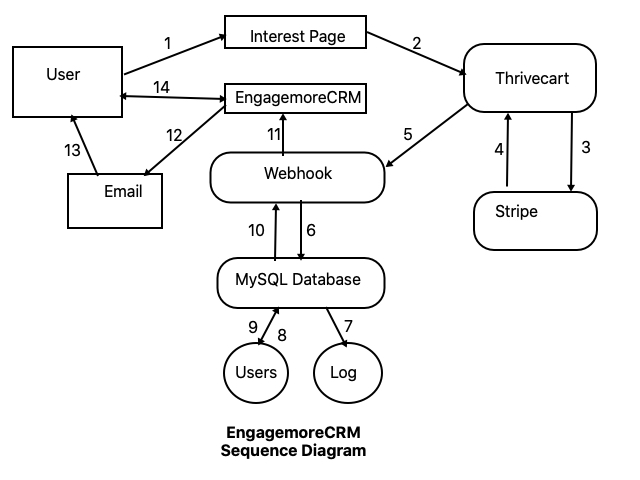
\includegraphics[width=6in]{EngagemoreCRM_Sequence.jpg}
\caption{\label{fig:sequence}Sequence Diagram}
\end{center}
\end{figure}
\begin{enumerate}
\item The user receives an invitation to a webpage where there is an ad for{\bf  EngagemoreCRM}.
\item The user clicks on a link on the page and is directed to
\item The {\bf Thrivecart} shopping page where there are different options. Selecting one and filling out the information sends encrypted credit card information to {\bf Stripe}, which handles it.
\item {\bf Stripe} returns a success code to {\bf Thrivecart} if the card is validated.
\item {\bf Thrivecart} the sends a webhook notification to the {\it webhook} application which services the event sent by {\bf Thrivecart}.  The {\it webhook} is located on an {\bf AWS EC2} instance located in Oregon and has the elastic ip of {\tt 44.231.61.194}.
\item The {\it webhook} examines the data received and checks that it contains the proper {\it API key} and {\it API user-id}.  
\item It then logs the data received to the {\bf MySQL database}, noting if it is a vaild request.
\item If the request is valid, the users {\bf email address} received from {\bf Thrivecart} is checked against the list of existing users in the {\it user database table}.
\item An existing users email is returned if it exists along with the users status.
\item {\bf MySQL} returns either the users email and status or a 'not found'.
\item The {\it webhook} examines the returned data from {\bf MySQL} and:
\begin{enumerate}
\item If the returned value is 'not found' we proceed to the next step.
\item if a users email was found and the status is {\bf inactive} a message is sent to {\bf EngagemoreCRM} to re-activate the suspended user as a payment has been received.  
\item Otherwise, if it is a payment, the action stops.  
\item If the event was a cancellation, then the message is sent to {\bf EngagemoreCRM} to suspend the user\footnote{An email is sent to {\it support@engagemorecrm.com} notifying that the account was cancelled} and the user is marked as inactive in the database.
\end{enumerate}
\item A message is sent to {\bf EngagemoreCRM} to add the user, and the {\it webhook} receives an {\bf EngagemoreCRM} user number in return.  That email and user number are added to the user database table and marked as 'active'.
\item {\bf EngagemoreCRM} then sends an email to the users email address inviting them to login with the password that is supplied.
\item The user then logs into {\bf EngagemoreCRM} and fills in needed information and begins to import contacts and set up their drips, etc.
\end{enumerate}

\noindent At the bottom and to the right and left of the MySQL database, are found:
\begin{enumerate}
\item Several reports that are obtained from the user table and logs table.  The monthly report provides a summary of new users, cancelled users, refunded users, etc.  Also, there is a small daily review that is examined for any break-in attempts or other unusual behavior.  The Special Monitoring Report runs periodically to detect transactions that are keyed to one or more individuals whose accounts might be having problems.
\item The Webhook is backed up remotely on a GitHub repository at: \\
https://github.com/woo37830/patti.git.  This contains the current operating version ( master ) and the development version ( develop ) and all of their histories.  The git log command will show this.
\item The MySQL database is backed up daily locally on the AWS EC2 instance using mysqldump.  Those backups are also copied to a remote site and saved.  Each day these are backup up to a separate device.
\end{enumerate}
\newpage
\begin{appendices}

\section{config.ini.php}
\noindent The config.ini.php page provides the externalized constants so that if the server address changes, it can be changed in one place.  Passwords are maintained here also, and thus this file is {\bf NOT} checked into the github\footnote{https://github.com} repository but are passed in by copying from the Trello\footnote{http://thrivecart.com} site where they are specified.

%\lstset{language=PHP,caption=config.ini.php,label=code:config}
\lstinputlisting{../config.fake}

\section{mysql\_common.php}
\noindent The file, mysql.comon.php, contains common mysql functions that all of the other files often share.  Such things as connect, logging to the logs database(see Table \ref{tab:logs}) getStatus, etc. are here.

%\lstset{language=PHP,caption=mysql\_common.php,label=code:common}
\lstinputlisting{../mysql_common.php}

\section{thrivecart\_api.php}
\noindent This page contains the logic to communicate the data received from the Thrivecart notification system to the EngagemoreCRM system.  The data and the specific EngagemoreCRM function will cause such actions as adding a user, changing their status from active to inactive, and changing the group in EngagemoreCRM to which they belong.

\lstinputlisting{../thrivecart_api.php}

\section{thrivecart.php}
\noindent This is the php page that is added to the Thrivecart site to receive the notifications when actions are taken in Thrivecart such as someone signing up, cancelling, etc.  It contains a switch statement that uses the event provided by Thrivecart to select the proper EngagemoreCRM API to perform the desired EngagemoreCRM action.  All notifications result in a logging event, and if the event is one supported by the webhook, then the proper API is invoked and the results are logged.  If a user is added, modified, or cancelled, the status is added or modified in the users(see Table \ref{tab:users}) data table.

\lstinputlisting{../thrivecart.php}

\section{utilities.php}
\noindent A set of functions used in tests and in the main thrivecart.php application.

\lstinputlisting{../utilities.php}

\section{add\_account.php}
\noindent The file, add\_account.php, handles the addition of the user who has just signed up through Thrivecart to the EngagemoreCRM system.  Depending upon which product they selected, the proper EngagemoreCRM group is selected and the data is added to the users table and marked as 'active'.

\lstinputlisting{../add_account.php}

\section{change\_account\_status.php}
\noindent Depending upon certain activities, the account status might be changed rom 'active' to 'inactive'.  This file provides the update function for that and communicates to EngagemoreCRM by either suspending or activating an account.

\lstinputlisting{../change_account_status.php}

\section{post\_api\_url.php}
\noindent This file was provided as a model by EngagemoreCRM to add users, change their status, etc. by the arguments provided.

\lstinputlisting{../post_api_url.php}

\section{upgrade\_account.php}
\noindent If the user decides to change their subscription, they can upgrade or downgrade their experiences in EngagemoreCRM.  This file handles those changes.

\lstinputlisting{../upgrade_account.php}

\section{git-info.php}
\noindent This file is provided to show, in certain cases the revision, branch, and database that is being used for particular transactions.  

\lstinputlisting{../git-info.php}

\end{appendices}
\end{document}
